\documentclass[aspectratio=169]{beamer}


\usepackage[utf8]{inputenc}
\usepackage{amsmath}
\usepackage{amsfonts}
\usepackage{amssymb}
\usepackage{graphicx}
\usepackage{ragged2e}  % `\justifying` text
\usepackage{booktabs}  % Tables
\usepackage{tabularx}
\usepackage{tikz}      % Diagrams
\usetikzlibrary{calc, shapes, backgrounds}
\usepackage{amsmath}
\usepackage{amssymb}
\usepackage{dsfont}
\usepackage{url}       % `\url
\usepackage{listings}  % Code listings
\usepackage[T1]{fontenc}
\usepackage{xcolor,colortbl}

\usepackage{theme/beamerthemehbrs}

\newcolumntype{C}{>{\centering\arraybackslash}m}
\newcolumntype{g}{>{\columncolor{gray}}c}

\author[H. Walli]{Hasnainali Walli}
\title{Lifelong Action Learning for Socially Assistive Robots}
%\subtitle{Subtitle of presentation}
\institute[HBRS]{Hochschule Bonn-Rhein-Sieg}
\date{November 25th, 2022}
\subject{Master's Thesis Defense}

% leave the value of this argument empty if the advisors
% should not be included on the title slide
\def\advisors{Prof. Dr. Paul G. Plöger, Prof. Dr. Sebastian Houben, Alex Mitrevski}

% \thirdpartylogo{path/to/your/image}


\begin{document}
{
\begin{frame}
\titlepage
\end{frame}
}


\section{Introduction}
%\subsection{A subsection}

\begin{frame}{Action Recognition}
      \framesubtitle{}%
\end{frame}

\begin{frame}{Lifelong Action Learning}
      \framesubtitle{}%
\end{frame}

\begin{frame}{Lifelong Action Learning}
      \framesubtitle{Application in CRI}%
\end{frame}

\begin{frame}{Lifelong Action Learning}
      \framesubtitle{Application in CRI}%
      \begin{figure}[h!]
      \centering
      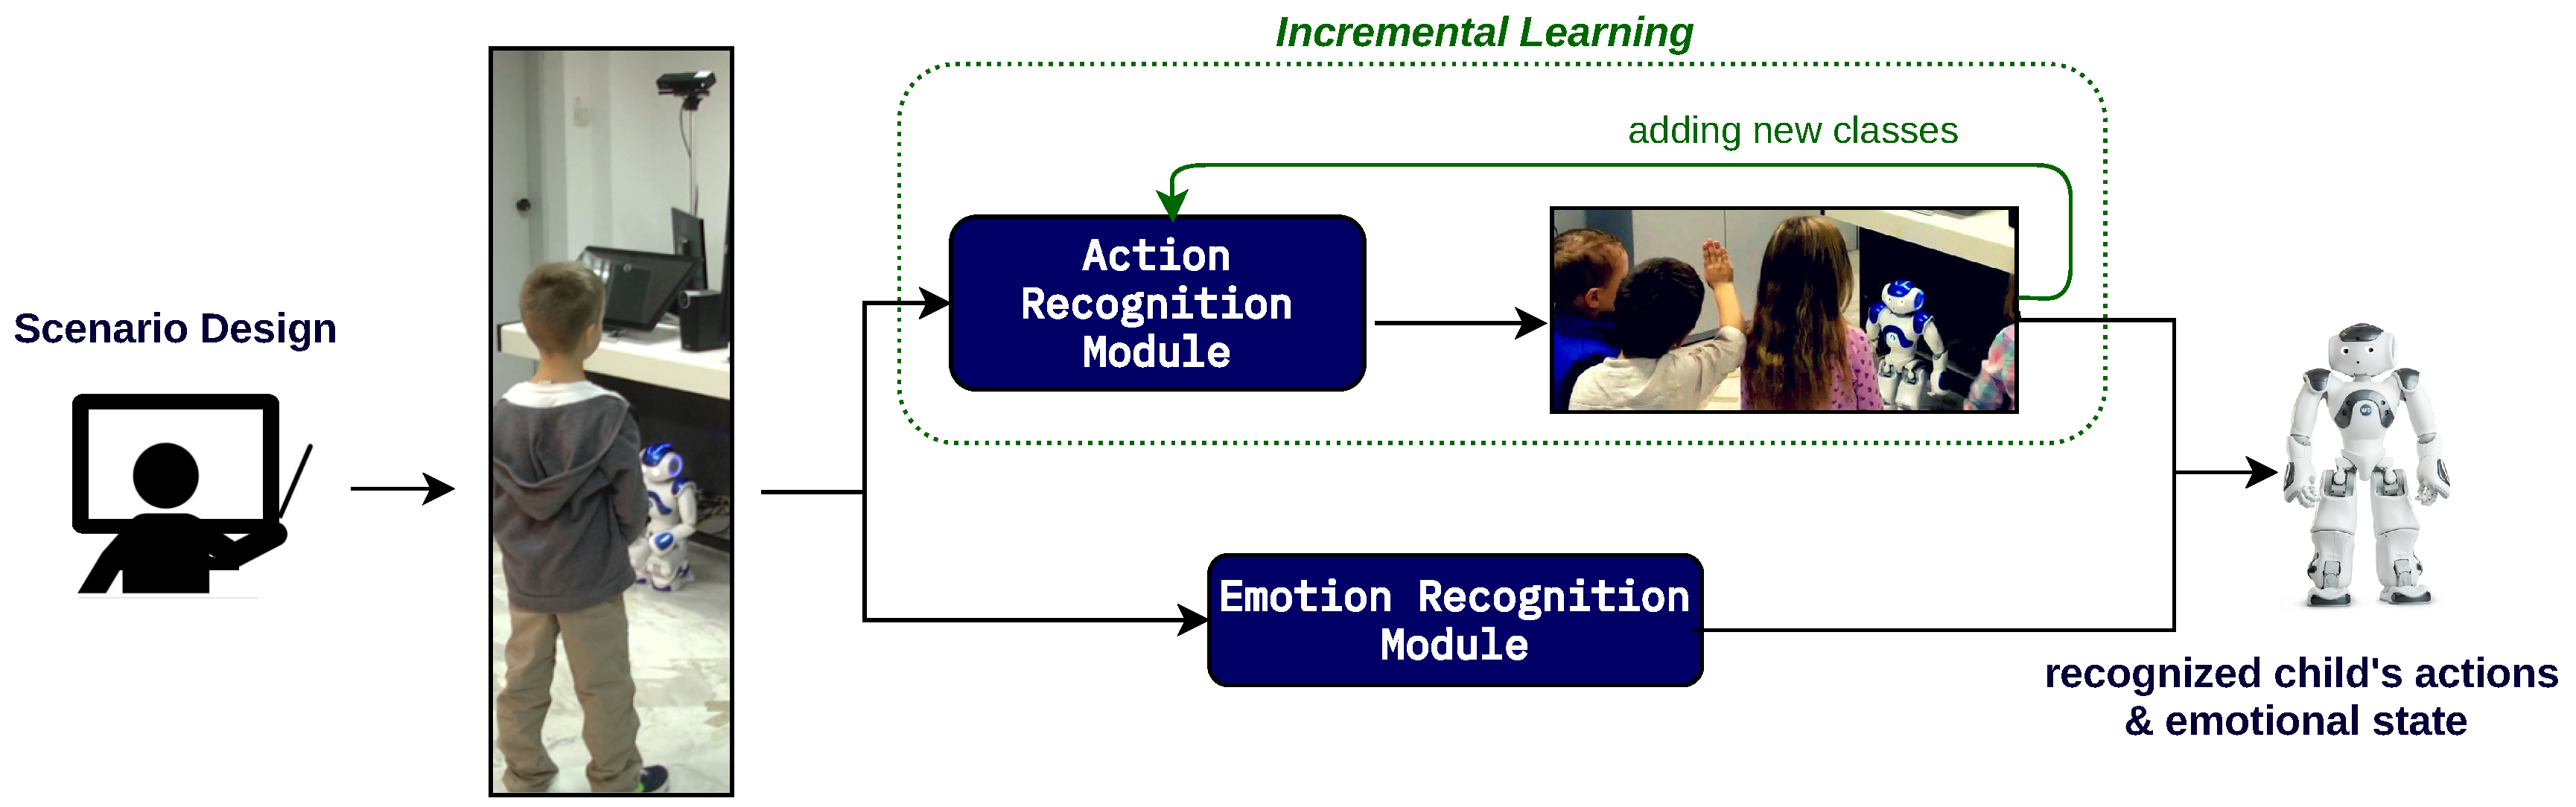
\includegraphics[width=0.9\textwidth]{images/IL_pipeline.png} 
      \caption{Incremental learning pipeline for action and emotion recognition. Source: \href{https://doi.org/10.3390/technologies9040086}{Visual Robotic Perception System with Incremental Learning for Child–Robot Interaction Scenarios}}
      \end{figure} 
\end{frame}

\begin{frame}{Lifelong Action Learning}
      \framesubtitle{Application in CRI}%
      
      \begin{figure}[h!]
      \centering
      \begin{tikzpicture}
              \draw[red,thick,dashed] (0,0) ellipse (3cm and 1cm);
              \node(a){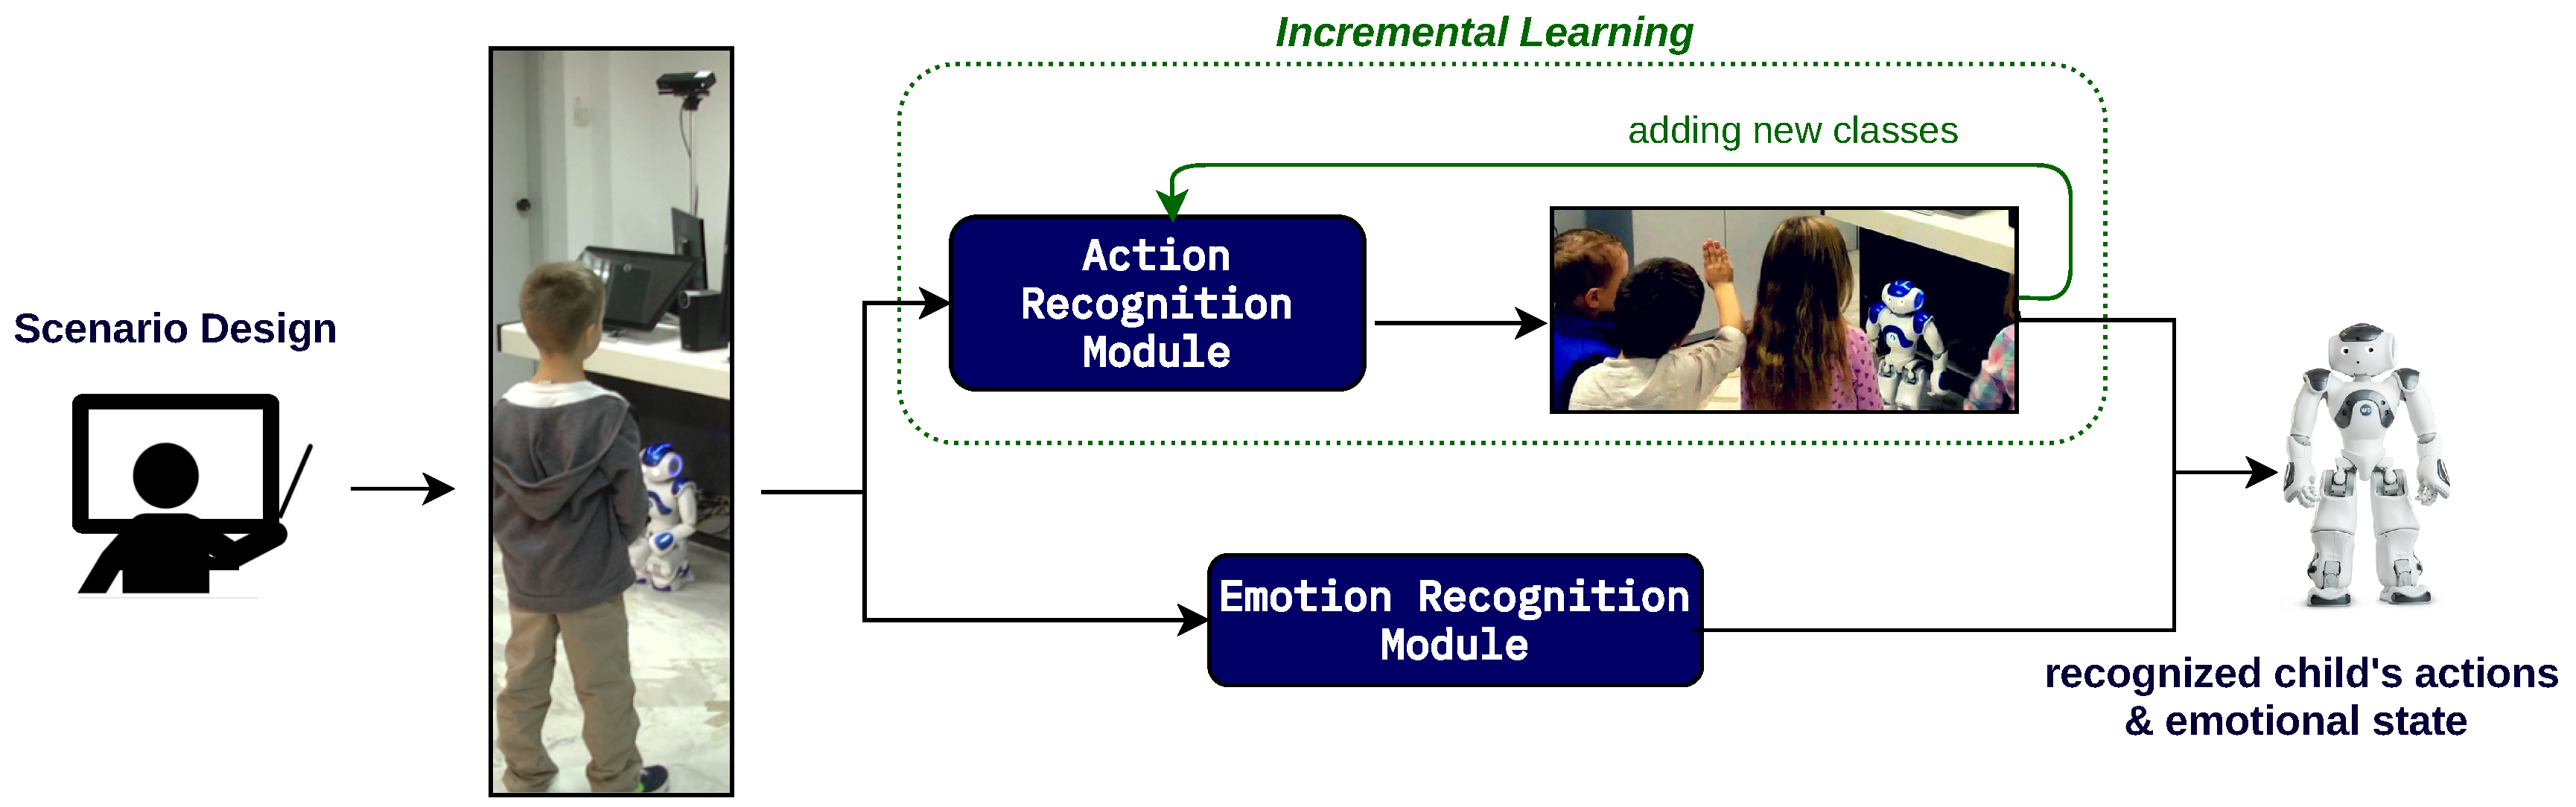
\includegraphics[width=0.9\textwidth]{images/IL_pipeline.png}};
              \node at (a.center) [draw, red, line width=3pt, ellipse, minimum width=200pt, minimum height=80pt, xshift=30pt, yshift=21pt]{};
      \end{tikzpicture}
      \caption{Incremental learning pipeline for action and emotion recognition Source: \href{https://doi.org/10.3390/technologies9040086}{Visual Robotic Perception System with Incremental Learning for Child–Robot Interaction Scenarios}}
      \end{figure} 
\end{frame}

\begin{frame}
      \framesubtitle{Application in CRI}%

      \begin{block}{~\vspace{0.7cm}}
      \begin{center}
      \vspace{-0.8cm}
      \begin{tabular}{p{0.45\textwidth}|p{0.45\textwidth}}
      \textcolor{white}{\bf Their Approach} & \textcolor{white}{\bf Our Approach} \\
      \begin{itemize}
              \item RGB+D and Optical Flow data
              \item TSN Network
              \item iCaRL Algorithm
              \item BabyRobot Dataset
      \end{itemize} &
      \begin{itemize}
              \item 3D Skeleton data
              \item CTR-GCN Network
              \item BiC Algorithm
              \item NTU RGB+D Dataset
      \end{itemize}\\ 
      \end{tabular}
      \end{center}
      \end{block}
\end{frame}

\begin{frame}{Our Approach}
      \framesubtitle{Methodology}%
      
      \begin{enumerate}
      \item Perform comparative analysis on skeleton-based action recognition networks
            \begin{itemize}
            \item CTR-GCN, MS-G3D, EfficientGCN, ViewAdaptive NN
            \item Joint, Bone and Joint Motions
            \item \textbf{Metrics}: Cross-Subject Accuracy, Training Time
            \end{itemize}
      \item Perform comparative analysis on class-incremental learning algorithms
            \begin{itemize}
            \item LwF, iCaRL, LUCIR, BiC
            \item 
            \item \textbf{Metrics}: Task-Aware \& Task-Agnostic Accuracy
            \end{itemize}
      \item Integrate final model on QTRobot
            \begin{itemize}
            \item 
            \item 
            \end{itemize}
      \end{enumerate}
\end{frame}

\section{Comparative Analysis: Action Recognition}

\begin{frame}{NTU Dataset}
      \framesubtitle{}%
      
      \vspace{-0.75cm}
      \begin{columns}
      \column{.4\textwidth}
      \begin{itemize}
            \item
            \item 
            \item 
      \end{itemize}
      
      \column{.6\textwidth}
      \begin{figure}[ht!]
            \centering
            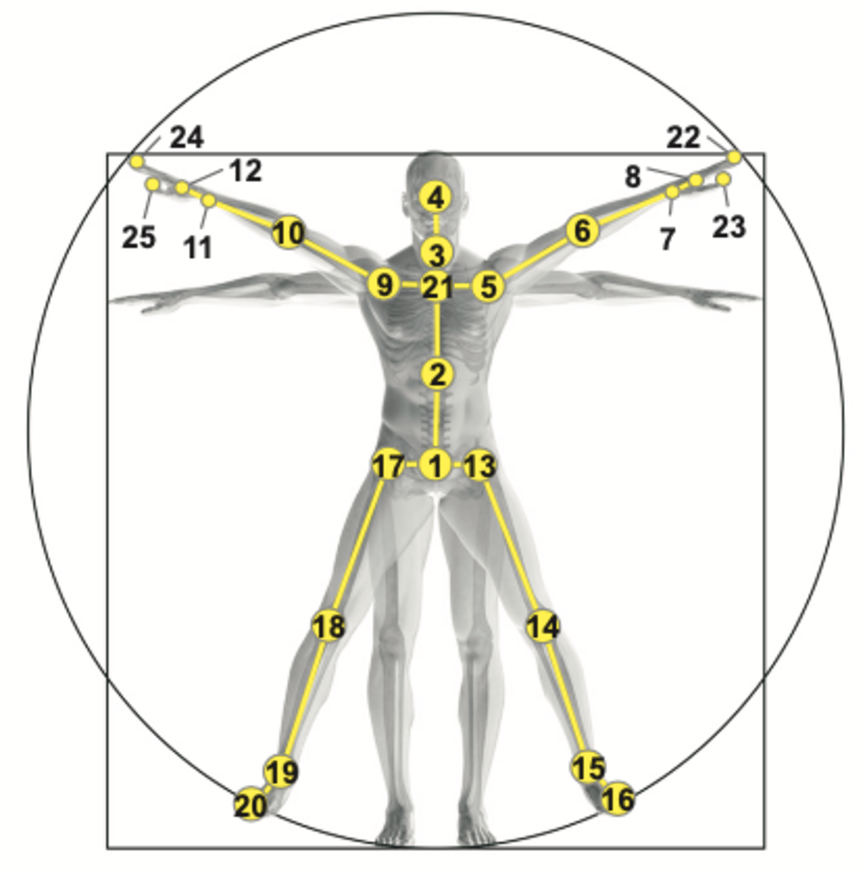
\includegraphics[width=0.7\textwidth]{images/joint_config.pdf}
            \caption{Human body joint configurations found in the NTU RGB-D dataset. Source: \href{https://doi.org/10.48550/arXiv.1604.02808}{NTU RGB+D: A Large Scale Dataset for 3D Human Activity Analysis}}
      \end{figure}      
      \end{columns}
\end{frame}

\begin{frame}{NTU Dataset}
      \framesubtitle{Subset of Actions}%
      
      \begin{table}[ht!]
      \centering
      \begin{tabular}{ |c|c|c|c| } 
              \hline
              Drink Water & Eat Meal & Brush Teeth & Drop \\ 
              \hline
              Pick Up & Throw & Sit Down & Stand Up \\ 
              \hline
              Clapping & Hand Waving & Kick Something & Hopping \\ 
              \hline
              Jump Up & Play with Phone/Tablet & Point to Something & Rub two Hands \\
              \hline
              Nod Head/Bow & Shake Head & Wipe Face & Cross Hands in Front \\
              \hline
      \end{tabular}
      \caption{Subset of action classes from the NTU RGB-D dataset}
      \end{table}
\end{frame}

\begin{frame}{Action Recognition Analysis Results}
      \framesubtitle{}%
      
      \begin{columns}
      \column{.6\textwidth}
      \begin{table}[h!]
      \centering
      {\small
      \begin{tabular}{ |C{0.35\textwidth}|C{0.25\textwidth}|C{0.2\textwidth}| } 
              \hline
              Network & Cross Subject & Cross View \\ 
              \hline
              CTR-GCN (Joint) & 92.63\% & 96.37\% \\ 
              \hline
              CTR-GCN (Bone) & 92.78\% & 96.02\% \\ 
              \hline
              CTR-GCN (Motion) & 92.51\% & 96.40\% \\ 
              \hline
              MS-G3D (Joint) & 91.27\% & 96.85\% \\ 
              \hline
              MS-G3D (Bone) & 90.90\% & 95.44\% \\ 
              \hline
              EfficientGCN-B4 (SG Layer) & 94.05\% & 97.47\% \\ 
              \hline
              EfficientGCN-B4 (EpSep Layer) & 94.43\% & 97.56\% \\ 
              \hline
              VA-NN (CNN) & 92.97\% & 92.20\% \\
              \hline
      \end{tabular}
      }
      \caption{Model Accuracy}
      \end{table}
      
      \column{.4\textwidth}
      \begin{table}[h!]
      \centering
      {\small
      \begin{tabular}{ |c|c| }
              \hline
              Network & Training Time \\
              \hline
              CTR-GCN & 4 hrs\\
              \hline
              MS-G3D & 8 hrs\\
              \hline
              EfficientGCN-B4 & 5 hrs\\
              \hline
              VA-NN (CNN) & 0.5 hrs\\
              \hline
      \end{tabular}
      }
      \caption{Model Training Time}     
      \end{table}
      \end{columns}
\end{frame}

\begin{frame}{Action Recognition Analysis Results}
      \framesubtitle{}%
      
      %\vspace{-0.25cm}
      \begin{table}[h!]
      \centering
      {\small
      \begin{tabular}{ | C{0.14\textwidth} | c | c | g | C{0.2\textwidth} | c | c | }
            \hline
            Action & CTR-GCN & MS-G3D &  & Action & CTR-GCN & MS-G3D \\
            \hline
            Drink Water & 82.48\% & 83.94\% & & Kick Something & 97.83\% & 94.93\% \\
            \hline
            Eat Meal & 78.91\% & 73.82\% & & Hopping & 98.91\% & 95.27\%  \\
            \hline
            Brush Teeth & 90.84\% & 91.21\% & & Jump Up & 98.91\% & 98.55\% \\
            \hline
            Drop & 90.18\% & 91.64\% & & Play with Phone/Tablet & 86.91\% & 90.91\% \\
            \hline
            Pick Up & 98.91\% & 94.55\% & & Point to Something & 92.39\% & 92.03\% \\
            \hline
            Throw & 96.36\% & 90.91\% & & Rub two Hands & 90.58\% & 89.49\% \\
            \hline
            Sit Down & 98.90\% & 97.80\% & & Nod Head/Bow & 96.01\% & 95.65\% \\
            \hline
            Stand Up & 98.17\% & 98.90\% & & Shake Head & 96.00\% & 95.64\% \\
            \hline
            Clapping & 82.42\% & 72.89\% & & Wipe Face & 92.39\% & 94.20\% \\
            \hline
            Hand Waving & 94.16\% & 94.89\% & & Cross Hands in Front & 93.84\% & 94.57\% \\
            \hline
      \end{tabular}
      }
      \caption{Cross-Subject accuracy results per class for CTR-GCN and MS-G3D models}
      \end{table}
\end{frame}

\section{Comparative Analysis: Class-Incremental Learning}

\begin{frame}{Incremental Learning}
      \framesubtitle{Concepts}%
\end{frame}

\begin{frame}{Incremental Learning}
      \framesubtitle{Performance Metrics}%
\end{frame}

\begin{frame}{Incremental Learning Analysis}
      \framesubtitle{Task Sequence}%
      
      \begin{table}[ht!]
      \centering
      {\small
      \begin{tabular}{ | c | C{0.17\textwidth} | g | c | C{0.17\textwidth} | g | c | C{0.17\textwidth} | }
            \hline
            Task \# & Action &  & Task \# & Action & & Task \# & Action \\
            \hline
            Task 1 & Wipe Face & & Task 5 & Pick Up & & Task 8 & Nod Head/Bow \\
            \hline
            & Eat Meal & & & Brush Teeth & & & Hopping \\
            \hline
            Task 2 & Cross Hands in Front & & Task 6 & Throw & & Task 9 & Drop \\
            \hline
            & Clapping & & & Point to Something & & & Drink Water \\
            \hline
            Task 3 & Kick Something & & Task 7 & Hand Waving & & Task 10 & Rub two Hands \\
            \hline
            & Shake Head & & & Stand Up & & & Jump Up \\
            \hline
            Task 4 & Sit Down & & & & & & \\
            \hline
            & Play with Phone/Tablet & & & & & & \\
            \hline
      \end{tabular}
      }
      \caption{Task sequence for class-IL comparative analysis}
      \end{table}
\end{frame}

\begin{frame}{}
      \framesubtitle{}%
\end{frame}

\begin{frame}{}
      \framesubtitle{}%
\end{frame}

\begin{frame}{}
      \framesubtitle{}%
\end{frame}

\begin{frame}{}
      \framesubtitle{}%
\end{frame}


    \begin{frame}[label=bibliography]{Bibliography}
      \framesubtitle{\TeX, \LaTeX, and Beamer}
      \begin{thebibliography}{9}
        \bibitem{knuth84}
            Donald~E.~Knuth.
            \emph{The \TeX book}.
            Addison-Wesley, 1984.
        \bibitem{lamport94}
            Leslie~Lamport.
            \emph{\LaTeX : A Document Preparation System}.
            Addison-Wesley, 1986.
        \bibitem{MG94}
            M.~Goossens, F.~Mittelbach, and A.~Samarin.
            \emph{The \LaTeX\ Companion}.
            Addison-Wesley, 1994.
        \bibitem{tantau04}
            Till~Tantau.
            \emph{User's Guide to the Beamer Class Version 3.01}.
            Available at \url{http://latex-beamer.sourceforge.net}.
        \bibitem{MS05}
            A.~Mertz and W.~Slough.
            Edited by B.~Beeton and K.~Berry.
            \emph{Beamer by example} In TUGboat,
              Vol. 26, No. 1., pp. 68-73.
      \end{thebibliography}
    \end{frame}



\end{document}
